\documentclass{article}
\usepackage[preprint]{neurips_2025}

\usepackage[utf8]{inputenc}
\usepackage[T1]{fontenc}
\usepackage{hyperref}
\usepackage{url}
\usepackage{microtype}
\usepackage{amsmath}
\usepackage{amssymb}
\usepackage{booktabs}
\usepackage{enumitem}
\usepackage{graphicx}
\usepackage{array}

\setlist[itemize]{leftmargin=*,itemsep=1pt,topsep=2pt,parsep=0pt,partopsep=0pt}
\setlength{\textfloatsep}{10pt plus 1pt minus 2pt}
\setlength{\floatsep}{8pt plus 1pt minus 2pt}
\setlength{\intextsep}{8pt plus 1pt minus 2pt}
\setlength{\abovecaptionskip}{4pt}
\setlength{\belowcaptionskip}{0pt}
\setlength{\bibsep}{0pt plus 0.3ex}

\title{Adaptive Evidence Acquisition for Grounded Video Question Answering}

\author{
  Aniket Salunke, Ketan More, Nazish Baliyan, Ritesh Thawkar \\
  Mohamed Bin Zayed University of Artificial Intelligence \\
  \{aniket.salunke,ketan.more,nazish.baliyan,ritesh.thawkar\}@mbzuai.ac.ae
}

\begin{document}
\maketitle

\begin{abstract}
Video question answering systems typically answer from a fixed visual context, although the evidence needed for a question may occupy only a few seconds of a much longer clip. This design hides two different failure modes: the model may spend computation on irrelevant frames, or it may answer correctly without selecting evidence that overlaps the annotated support moment. We formulate grounded VideoQA as \emph{adaptive evidence acquisition}. A policy selects frame and temporal-segment evidence from a candidate pool before a vision-language answerer predicts the multiple-choice answer, making answer accuracy, acquisition cost, and temporal grounding jointly measurable. Our study on NExT-GQA uses controlled answerer swaps to separate evidence-selection quality from visual reasoning quality. A frozen CLIP-style answerer validates the pipeline but saturates near 0.39 accuracy, while Qwen2.5-VL exposes the intended tradeoff. A lightweight MLP router with temporal non-maximum suppression (NMS) reaches 0.689 test Acc@QA and 0.321 Acc@GQA at cost 2.935, improving substantially over one-segment evidence at 0.668 Acc@QA and 0.221 Acc@GQA. A fixed 3-frame + 3-segment reference reaches 0.724 Acc@QA and 0.454 Acc@GQA, but costs 7.5. Oracle top-2 evidence reaches 0.442 Acc@GQA at cost 2.493, showing that the candidate pool contains compact supporting evidence and that the remaining gap is primarily routing quality. These results support a Pareto view of grounded VideoQA: compact learned evidence is efficient, but faithful temporal grounding must be measured directly rather than inferred from answer accuracy.
\end{abstract}

\section{Introduction}
Video question answering (VideoQA) requires a system to answer natural-language questions about events, objects, interactions, and causal relations in a video. Unlike image VQA, the evidence is distributed over time: the answer may depend on an action that happens briefly, an object that appears only once, or a causal relation between two nearby events. This temporal structure makes VideoQA both a recognition problem and an evidence-localization problem. A model can output the correct option by exploiting language priors, broad scene context, or correlations in the answer choices, but such an answer is less trustworthy if the system cannot show that it used the moment that actually supports the response.

Most practical VideoQA pipelines simplify this issue by choosing a fixed visual context: a fixed number of frames, a fixed number of clips, or the top-$K$ retrieved snippets. This is convenient for batching and model design, but it treats all questions as if they require the same amount of evidence. In grounded VideoQA, that assumption is especially problematic. Some questions can be answered from one short action; others require comparing events before and after a state change. A fixed budget may therefore be too expensive for easy questions and too weakly grounded for difficult ones.

We study this issue as adaptive evidence acquisition. Rather than always giving the answerer the same number of frames and video segments, we construct a candidate evidence pool and let a policy choose evidence before stopping. The selected evidence is then passed to an answerer. This formulation turns ``how much context is enough?'' into an empirical question and exposes the tradeoff between three quantities: answer accuracy, evidence cost, and temporal grounding. The same framework can express a low-cost one-segment setting, a compact learned router with diversity filtering, a temporally supervised diagnostic router, oracle evidence selection, and a larger fixed-budget setting that favors temporal coverage.

The central experimental design choice is to separate evidence selection from answer generation. We first evaluate policies with a frozen CLIP-based answerer to obtain cheap, reproducible controls over evidence budget. These controls reveal that the frozen answerer is a bottleneck: temporal coverage improves as more evidence is selected, but answer accuracy changes only slightly. We then keep the evidence selections fixed and replace only the answerer with Qwen2.5-VL-3B-Instruct \citep{qwen2025vl}. If accuracy improves under the same evidence, the failure was visual reasoning; if grounding remains poor, the failure is evidence selection. This controlled swap is what lets the results support a research claim rather than only a stronger-model result.

Our experiments are organized around three questions. First, does selecting a small amount of question-conditioned evidence improve grounding over a single low-cost segment? Second, does a weak frozen answerer hide the value of better evidence? Third, when a stronger VLM is used, how much of the gap to a larger fixed budget can be closed by learned routing rather than simply increasing visual context? The answer is not a single winner. The MLP+NMS router is the strongest learned grounded operating point, the temporal-supervised router is cheaper but localizes less faithfully under IoU, and oracle evidence nearly matches the fixed 3+3 reference at much lower cost. This is the core result: grounded VideoQA should be reported as a Pareto tradeoff rather than as answer accuracy alone.

\paragraph{Contributions.}
This work makes four contributions centered on grounded VideoQA pipeline design and controlled evidence-budget evaluation:
\begin{itemize}
  \item We formulate NExT-GQA as a budgeted evidence-acquisition problem over frame and short temporal segment evidence.
  \item We implement one-segment, linear-policy, MLP-router, temporal-diversity, temporal-supervised, oracle, and fixed-budget evidence selectors under a common candidate-pool representation.
  \item We evaluate the same selected evidence under both a frozen CLIP-style answerer and a stronger Qwen2.5-VL answerer.
  \item We report accuracy, evidence cost, evidence count, temporal overlap, and grounded answer accuracy, showing that MLP+NMS is the best learned grounded selector while oracle evidence exposes substantial headroom in the candidate pool.
\end{itemize}

\section{Related Work}
Early VideoQA benchmarks such as MovieQA \citep{tapaswi2016movieqa}, TGIF-QA \citep{jang2017tgifqa}, and TVQA \citep{lei2018tvqa} established video reasoning as a multimodal problem involving temporal visual content and language. These datasets moved the field beyond static object recognition: systems must identify actions, track interactions, and connect visual events to natural-language questions. They also exposed a modeling tension that remains important here. Sampling a few frames can be efficient, but it can miss the temporal evidence needed for action and causal questions; processing dense video context can improve coverage, but it is expensive and can introduce irrelevant information. Our evidence pool uses both frames and short segments to study this tradeoff directly.

Grounded VideoQA adds an explicit faithfulness requirement. TVQA+ \citep{lei2019tvqaplus} extended TVQA with spatio-temporal evidence annotations, making clear that a correct answer alone is not enough when the goal is interpretable video understanding. NExT-QA \citep{xiao2021nextqa} emphasized temporal and causal questions, and NExT-GQA further asked whether a model's answer is supported by temporally grounded visual evidence \citep{xiao2023trust}. This distinction is central to this work. We do not only ask whether the answer letter is correct; we also measure whether the selected evidence overlaps the annotated support span. The gap between Acc@QA and Acc@GQA in our results shows that answer correctness and grounding correctness can diverge substantially.

Pretrained vision-language models changed the practical design of VideoQA systems. CLIP \citep{radford2021clip}, VideoCLIP \citep{xu2021videoclip}, and CLIP4Clip \citep{luo2021clip4clip} made text-image and text-video alignment practical at scale, enabling retrieval and scoring pipelines that can be built without training a full VideoQA model from scratch. Later systems showed that strong VideoQA performance can be obtained by combining pretrained visual encoders, frozen or lightly adapted language models, and retrieval-style context construction \citep{yang2021justask,yang2022frozenbilm,pan2023r2a}. These systems motivate our use of pretrained encoders and VLMs. At the same time, our frozen-answerer experiments show a risk in this design space: if the answerer is too weak, improvements in evidence selection may not appear as improvements in answer accuracy. This motivates our controlled comparison between a frozen scorer and Qwen2.5-VL.

Recent retrieval-augmented video work focuses on long videos and selective context construction \citep{luo2024videorag,gia2025vrag}. This literature reinforces the budget question: once a large candidate pool exists, the system still needs to select a compact subset before answering. However, many retrieval-augmented systems report downstream answer quality without explicitly charging evidence cost or measuring whether the selected evidence is temporally aligned with ground truth. Our contribution is narrower but more diagnostic. We hold the evidence selections fixed, swap the answerer, and report answer accuracy, cost, and grounding under the same protocol. This lets us ask whether the bottleneck is evidence acquisition or answer generation, a distinction that is often hidden when retrieval and generation are optimized as a single black-box pipeline.

\section{Problem Statement}
Let a grounded VideoQA example be
\[
  x = (v, q, \mathcal{A}, y, \mathcal{T}),
\]
where $v$ is a video, $q$ is a question, $\mathcal{A}=\{a_1,\ldots,a_K\}$ is the set of answer options, $y$ is the correct option index, and $\mathcal{T}$ is the annotated temporal grounding span when available. From the video we construct a candidate evidence pool
\[
  \mathcal{E}(x)=\{e_1,\ldots,e_N\}.
\]
Each evidence item $e_i$ has a modality $m_i$ (frame or segment in our NExT-GQA experiments), a time interval $I_i=[s_i,t_i]$, a retrieval score $r_i$, and an acquisition cost $c_i$. A policy selects a subset $S \subseteq \mathcal{E}(x)$ with total cost
\[
  C(S)=\sum_{e_i \in S} c_i.
\]
An answerer $f_\phi$ receives $(q,\mathcal{A},S)$ and predicts $\hat{y}=f_\phi(q,\mathcal{A},S)$.

The goal is to find an evidence-selection strategy that achieves high answer accuracy while keeping $C(S)$ small and maintaining temporal overlap with $\mathcal{T}$. A simplified objective is:
\[
  \max_{\pi} \; \mathbb{E}_{x}\left[
    \mathbf{1}\{f_\phi(q,\mathcal{A},S_\pi)=y\}
    - \lambda C(S_\pi)
    + \beta G(S_\pi,\mathcal{T})
  \right],
\]
where $S_\pi$ is the evidence selected by policy $\pi$ and $G$ measures grounding overlap. In this work, we do not train the full VLM and evidence policy end-to-end against this objective. Instead, we compare explicit operating points: low-cost one-segment evidence, a linear learned policy, an MLP router with temporal diversity filtering, a temporally supervised diagnostic router, oracle selection from the same pool, and a higher-cost fixed-budget reference.

This formulation gives three evaluation axes. Acc@QA measures whether the final answer is correct. Cost measures how much visual context the system consumes. Grounding measures whether the selected evidence actually covers the annotated support event. A method can improve one axis while hurting another: for example, adding many segments can improve coverage while increasing cost, and a stronger answerer can improve Acc@QA without changing temporal overlap. We therefore treat the desired behavior as a Pareto tradeoff rather than a single scalar leaderboard number.

\section{Proposed Method}
\subsection{Evidence Pool Construction}
The pipeline first normalizes NExT-GQA annotations into a unified schema containing question text, answer options, answer labels, video metadata, and temporal grounding spans. For each example, we sample frame candidates and construct short temporal segment candidates. Frame evidence is represented by extracted image artifacts, while segment evidence is represented by a video interval and, for VLM answering, one sampled frame from that interval. Each candidate stores its time interval, modality, retrieval score, and metadata needed to reconstruct the selected evidence at inference time.

We use a deliberately simple cost model: frames have cost 1.0 and segments have cost 1.5. The exact units are abstract, but the relative scale encodes the fact that a segment covers more temporal context than a single frame and should be charged more heavily. This cost model is useful because it makes the comparison between policies explicit. A one-segment method costs 1.5, compact learned selectors cost roughly 2.3--3.0 depending on how many frames and segments they choose, and the fixed 3+3 reference costs 7.5. The reported improvements can therefore be read as accuracy or grounding gained per unit of acquired evidence rather than as raw accuracy alone.

\begin{figure}[t]
  \centering
  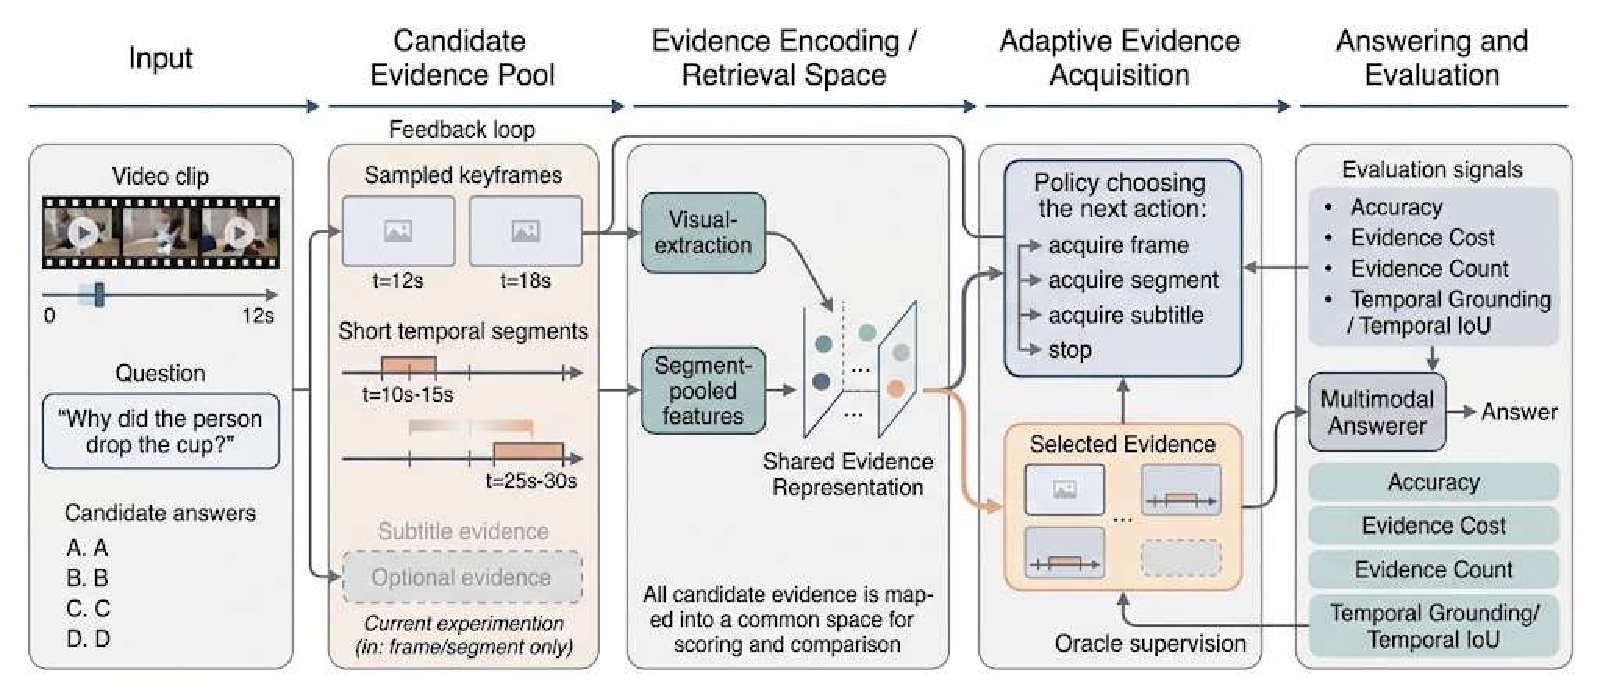
\includegraphics[width=0.95\linewidth]{figure_1.pdf}
  \caption{Adaptive evidence-acquisition pipeline. We normalize NExT-GQA examples, construct frame and segment candidates, select evidence under a budget, answer using either a frozen scorer or Qwen2.5-VL, and evaluate answer accuracy, cost, and temporal grounding.}
  \label{fig:pipeline}
\end{figure}

\subsection{Evidence Policies}
We evaluate a ladder of evidence policies that share the same candidate pool. The one-segment policy selects the highest-scoring segment and stops. It is a strong low-cost control because it gives the answerer a short temporal context at cost 1.5. The linear learned policy is a sequential controller trained from oracle traces exported from the frozen multimodal answerer; it selects two evidence items before stopping. This row is retained as a historical learned-policy baseline because it was the first compact selector that improved grounding over one segment.

Our main learned selector is a lightweight MLP router. It scores each frame and segment candidate using retrieval score, modality, temporal location, duration, question-conditioned features, and budget-related features. At inference time, the router selects the top two candidates. We also apply temporal NMS over candidate intervals to discourage redundant evidence: if two high-scoring candidates overlap too strongly, the selector keeps the stronger one and moves to the next non-overlapping candidate. This produces the MLP+NMS operating point reported as the main learned method.

We include two diagnostic selectors. The temporal-supervised router is an MLP trained directly from temporal-overlap labels over the retrieved pool. It tests whether explicit temporal supervision improves routing, but it is reported as an ablation because its training signal optimizes overlap rather than final grounded QA. The oracle selector chooses the top candidates by ground-truth temporal IoP from the same candidate pool. It is not a deployable method; it measures how much support is already present in the pool and how much headroom remains for better routing.

The fixed policies select a predetermined number of frames and segments. The fixed 3+3 reference selects three frames and three segments, producing a much larger evidence set with cost 7.5. If a compact selector is close to fixed 3+3 in answer accuracy but much cheaper, then it is an efficient operating point. If it remains far below fixed 3+3 in Acc@GQA, then the missing component is temporal coverage rather than answer generation. This is the main diagnostic role of the fixed-budget ladder.

\subsection{Answerers}
We use two answerer families. The first is a frozen multimodal scorer based on CLIP-style visual and text features. It is cheap and reproducible, making it useful for sweeping evidence policies, but our diagnostics showed that it was not strong enough for final claims. The second is Qwen2.5-VL-3B-Instruct \citep{qwen2025vl}. For each example, selected visual evidence is converted into an ordered list of images, and the model receives a multiple-choice prompt asking it to output one answer letter. We parse the first valid option letter from the generation and count malformed outputs as parse failures; in the completed Qwen runs the parse failure rate is zero.

We use deterministic decoding with a short generation length so that differences reflect selected evidence rather than sampling noise. For batched inference, the tokenizer is set to left padding, and the runner falls back to smaller batches on GPU out-of-memory errors. This was necessary to use the 24GB GPU efficiently while preserving valid generations. Importantly, Qwen is used only as the answerer in these experiments; the evidence selections are produced independently, which keeps the answerer ablation controlled.

\subsection{Evaluation Metrics}
We report standard answer accuracy (Acc@QA), average evidence cost, and average evidence count. For grounding, we compute intersection over prediction (IoP) and intersection over union (IoU) between selected evidence intervals and the ground-truth temporal span. For selected evidence $S$ and target span $\mathcal{T}$, we report the best overlap over selected items:
\[
  \mathrm{IoP}(S,\mathcal{T}) = \max_{e_i \in S}
  \frac{|I_i \cap \mathcal{T}|}{|I_i|},
  \quad
  \mathrm{IoU}(S,\mathcal{T}) = \max_{e_i \in S}
  \frac{|I_i \cap \mathcal{T}|}{|I_i \cup \mathcal{T}|}.
\]
Finally, Acc@GQA counts an example as correct only if the answer is correct and $\mathrm{IoP}\geq 0.5$. This is an approximate paper-style grounded QA metric because it uses the best selected evidence item rather than an official single-window evaluator.

The distinction between IoP and IoU matters for our evidence sets. IoP asks whether a selected item is mostly inside the annotated support window, while IoU penalizes both under-coverage and over-coverage relative to the target span. We emphasize Acc@GQA with IoP@0.5 because it directly asks whether a correct answer is supported by at least one sufficiently aligned selected evidence item. We still report IoU metrics to make the temporal-localization behavior transparent.

\section{Experimental Setup}
\paragraph{Dataset.}
We evaluate on NExT-GQA, a grounded VideoQA benchmark derived from NExT-QA. The full validation split used here contains 3,358 examples. The test split contains 5,553 examples. All Qwen rows reported in the main comparison and router ablations are completed full-test results. Fixed 3+3 is retained as a high-cost coverage reference rather than as the proposed method.

\paragraph{Baselines and controls.}
The frozen-answerer experiments include one-segment, linear learned two-item, fixed 3-frame + 3-segment, and fixed 6-frame + 6-segment controls. The Qwen experiments evaluate one-segment evidence, linear policy evidence, MLP top-2 evidence, MLP+NMS evidence, the temporal-supervised router, oracle top-2 evidence, oracle top-3 evidence, and fixed 3+3 evidence. This gives a low-cost control, multiple compact learned selectors, oracle headroom estimates, and a high-cost coverage reference.

\paragraph{Implementation details.}
Frame artifacts are extracted from source videos and cached. CLIP features are precomputed for the frozen answerer and retrieval controls. Qwen2.5-VL inference uses one sampled image for each selected segment and the selected frame image for each selected frame. The final Qwen test runs use batch size 32 for one-segment evidence, 16 for compact two-item evidence, and 4 for fixed 3+3 evidence. The experiments run on a single 24GB Quadro RTX 6000 GPU.

\paragraph{Ablations.}
We isolate evidence modality, evidence budget, answerer strength, router architecture, temporal diversity, and oracle headroom. The modality/budget ablations use the frozen answerer because they are cheap enough to run over many fixed allocations. The Qwen router ablations reuse selected evidence files and swap only the evidence selector, while keeping the final answerer fixed. This separates the effect of routing from the effect of answer generation.

\paragraph{Statistical reporting.}
For the main test comparisons, we compute 1,000-sample bootstrap confidence intervals over examples. These intervals are most useful for answer accuracy because the Qwen answerer changes answer predictions while the evidence selector remains fixed. For grounding-only quantities, confidence intervals reflect variation in selected temporal overlap across examples rather than model stochasticity.

\section{Results and Discussion}
\subsection{Main Comparison With Published NExT-GQA Methods}
Table~\ref{tab:main-comparison} is the main results table. It places our operating points next to representative published NExT-GQA results. The prior rows report official test-set numbers from the NExT-GQA and QGAC-TR papers \citep{xiao2023trust,xu2024qgac}. Our Qwen rows are completed test results. The comparison should therefore be read as protocol context, not as a formal leaderboard replacement: prior methods output a single localized span under the official evaluator, whereas our grounding metrics use the selected evidence set and the best-overlap protocol described above. Evidence cost is reported for our methods and left unspecified for prior work because it is not reported under the same acquisition-cost model.

Even with that caveat, the table is useful. Published methods show the standard pattern for grounded VideoQA: Acc@QA can be high while Acc@GQA remains much lower. Reporting mIoP, IoP@0.5, mIoU, and IoU@0.5 makes the grounding behavior visible rather than hiding it inside Acc@GQA. Our Qwen one-segment row is the low-cost control. The MLP+NMS row is the proposed learned operating point: it improves Acc@GQA from 0.221 to 0.321 over one segment while keeping cost below 3.0. The oracle and fixed rows then show the remaining gap: the pool contains enough compact evidence to approach the high-cost reference, but the learned router does not yet recover all of it.

\begin{table}[t]
  \centering
  \scriptsize
  \setlength{\tabcolsep}{2pt}
  \caption{Main comparison with published NExT-GQA results. Prior rows use official test metrics; our grounding metrics use selected-evidence best overlap. MLP+NMS is the proposed learned selector; oracle and fixed 3+3 are diagnostic references.}
  \label{tab:main-comparison}
  \resizebox{\linewidth}{!}{%
  \begin{tabular}{@{}lrrrrrrr@{}}
    \toprule
    Method & Acc@QA & Acc@GQA & mIoP & IoP@0.5 & mIoU & IoU@0.5 & Cost \\
    \midrule
    Temp[CLIP] NG+ \citep{xiao2023trust} & 0.602 & 0.160 & 0.257 & 0.255 & 0.121 & 0.089 & -- \\
    FrozenBiLM NG+ \citep{xiao2023trust} & 0.708 & 0.175 & 0.242 & 0.237 & 0.096 & 0.061 & -- \\
    SeViLA \citep{xiao2023trust} & 0.681 & 0.166 & 0.295 & 0.229 & 0.217 & 0.138 & -- \\
    QGAC-TR \citep{xu2024qgac} & 0.636 & 0.183 & 0.283 & 0.277 & 0.157 & 0.117 & -- \\
    \midrule
    Qwen one segment control & 0.668 & 0.221 & 0.301 & 0.311 & 0.165 & 0.133 & 1.500 \\
    Qwen MLP+NMS (Our) & 0.689 & 0.321 & 0.440 & 0.453 & 0.246 & 0.210 & 2.935 \\
    \midrule
    Qwen oracle top-2 reference & 0.701 & 0.442 & 0.618 & 0.615 & 0.224 & 0.207 & 2.493 \\
    Qwen fixed 3 frames + 3 segments reference & 0.724 & 0.454 & 0.618 & 0.615 & 0.296 & 0.287 & 7.500 \\
    \bottomrule
  \end{tabular}
  }
\end{table}

\subsection{Frozen Answerer Controls}
Table~\ref{tab:frozen-test} reports full NExT-GQA test results for the frozen answerer. The learned two-item policy improves grounding over the one-segment policy, raising Acc@GQA from 0.124 to 0.164, but answer accuracy remains close to 0.38 for all compact evidence settings. The fixed 6+6 control has the best grounding because it covers more video time, but it costs almost ten times more than a single segment. These results show that policy design alone is not sufficient when the answerer is weak.

This result is important for interpreting the rest of the paper. If we only evaluated the frozen answerer, the conclusion would be that evidence acquisition barely matters for answer accuracy. The grounding metrics show that this is false: larger budgets and the learned two-item policy do select more temporally relevant evidence. The missing link is that the frozen scorer is too weak to translate that evidence into better answers. This motivates the Qwen experiments in Table~\ref{tab:qwen-router}.

\begin{table}[t]
  \centering
  \scriptsize
  \caption{Frozen-answerer results on the NExT-GQA test split.}
  \label{tab:frozen-test}
  \begin{tabular}{lrrrrrrrr}
    \toprule
    Method & Acc@QA & Cost & Count & mIoP & IoP@0.5 & mIoU & IoU@0.5 & Acc@GQA \\
    \midrule
    One segment & 0.378 & 1.500 & 1.000 & 0.301 & 0.311 & 0.165 & 0.133 & 0.124 \\
    Learned policy, two items & 0.381 & 2.795 & 2.000 & 0.403 & 0.410 & 0.206 & 0.181 & 0.164 \\
    Fixed 3 frames + 3 segments & 0.388 & 7.500 & 6.000 & 0.618 & 0.615 & 0.296 & 0.287 & 0.245 \\
    Fixed 6 frames + 6 segments & 0.394 & 14.908 & 11.939 & 0.784 & 0.787 & 0.412 & 0.446 & 0.316 \\
    \bottomrule
  \end{tabular}
\end{table}

\subsection{Qwen Test Router Results}
Table~\ref{tab:qwen-router} reports the completed full-test Qwen2.5-VL results for the compact selectors and diagnostic references. Qwen substantially changes the interpretation of evidence selection. With one segment, answer accuracy is already high at 0.668, but grounded answer accuracy is only 0.221. The linear two-item policy improves Acc@GQA to 0.297, showing that compact evidence selection is useful once the answerer is strong enough. The MLP router improves further, and adding temporal NMS gives the best learned grounded result: 0.321 Acc@GQA at cost 2.935.

The temporal-supervised router is informative but not the main method. It is cheaper and has slightly higher answer accuracy than MLP+NMS, but its mIoU is only 0.088 because it often selects short frame-like evidence that is inside the support moment without covering much of the annotated span. This confirms why IoP and IoU should both be reported. IoP captures whether selected evidence is support-compatible, while IoU exposes under-coverage. The oracle rows show the available headroom: oracle top-2 reaches 0.442 Acc@GQA at cost 2.493, close to fixed 3+3 at 0.454 despite using one third of the evidence cost.

\begin{table}[t]
  \centering
  \scriptsize
  \caption{Completed NExT-GQA test results with Qwen2.5-VL. MLP+NMS is the strongest learned grounded selector. The temporal-supervised router is a diagnostic ablation, and oracle rows measure candidate-pool headroom.}
  \label{tab:qwen-router}
  \resizebox{\linewidth}{!}{%
  \begin{tabular}{lrrrrrrrr}
    \toprule
    Method & Acc@QA & Cost & Count & mIoP & IoP@0.5 & mIoU & IoU@0.5 & Acc@GQA \\
    \midrule
    One segment & 0.668 & 1.500 & 1.000 & 0.301 & 0.311 & 0.165 & 0.133 & 0.221 \\
    Linear policy, min 2 & 0.696 & 2.795 & 2.000 & 0.403 & 0.410 & 0.206 & 0.181 & 0.297 \\
    MLP top-2 & 0.687 & 3.000 & 2.000 & 0.407 & 0.423 & 0.238 & 0.213 & 0.301 \\
    MLP+NMS & 0.689 & 2.935 & 2.000 & 0.440 & 0.453 & 0.246 & 0.210 & 0.321 \\
    Temporal-supervised router & 0.696 & 2.273 & 2.000 & 0.433 & 0.432 & 0.088 & 0.075 & 0.312 \\
    Oracle top-2 & 0.701 & 2.493 & 2.000 & 0.618 & 0.615 & 0.224 & 0.207 & 0.442 \\
    Oracle top-3 & 0.710 & 3.793 & 3.000 & 0.618 & 0.615 & 0.278 & 0.268 & 0.448 \\
    Fixed 3 frames + 3 segments & 0.724 & 7.500 & 6.000 & 0.618 & 0.615 & 0.296 & 0.287 & 0.454 \\
    \bottomrule
  \end{tabular}
  }
\end{table}

Figure~\ref{fig:tradeoff} visualizes the same Qwen test results as a cost tradeoff. The left panel shows that answer accuracy is relatively flat among compact selectors, while the right panel shows much larger differences in grounded answer accuracy. This is the central empirical point: answer accuracy alone would make one segment, linear policy, MLP+NMS, and temporal routing look similar, but the grounding metrics reveal different evidence behavior.

\begin{figure}[t]
  \centering
  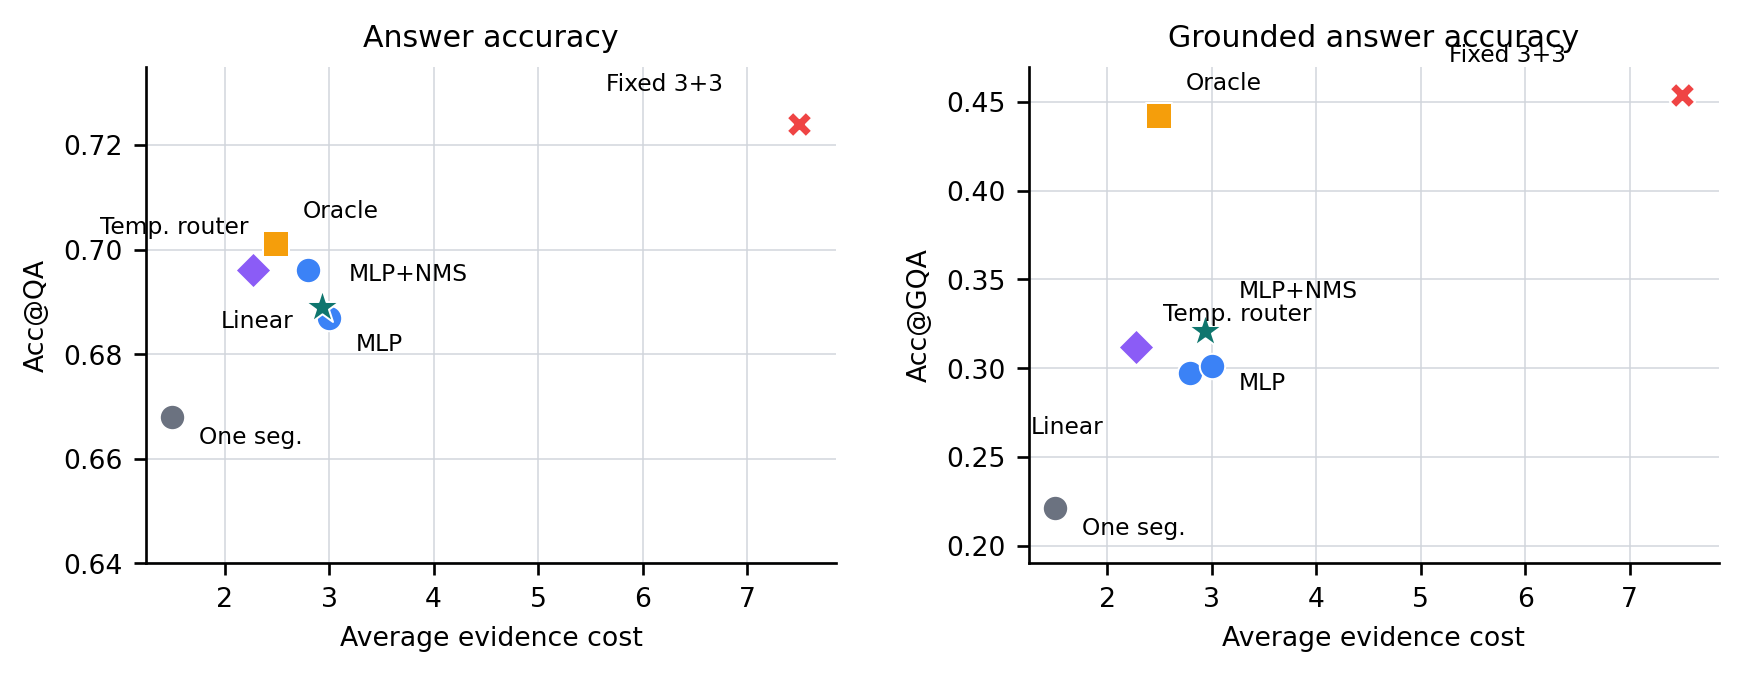
\includegraphics[width=0.95\linewidth]{qwen_current_tradeoff_presentation.png}
  \caption{Qwen test tradeoff for answer accuracy and grounded answer accuracy as evidence cost increases. MLP+NMS is the strongest learned grounded selector; oracle top-2 shows that compact evidence in the pool can nearly match the high-cost fixed reference.}
  \label{fig:tradeoff}
\end{figure}

The key comparison is between one segment, MLP+NMS, oracle top-2, and fixed 3+3. MLP+NMS costs 2.935 instead of 1.5, but it improves grounded accuracy by 10.0 points over one segment. Compared with fixed 3+3, it keeps about 95\% of the answer accuracy while using only 39\% of the evidence cost. Oracle top-2 then shows that the candidate pool itself is not the main bottleneck: it reaches 97\% of the fixed-reference Acc@GQA while using 33\% of the cost. The remaining challenge is to close the router gap without expanding the evidence budget.

\subsection{Ablations}
The frozen budget sweep confirms that larger fixed evidence sets improve temporal coverage, but the frozen answerer barely converts that evidence into higher answer accuracy. The more important ablation is therefore candidate-pool quality versus routing quality. Table~\ref{tab:pool-ablation} shows that support increases steadily from one to six available candidates, and the @6 row matches the temporal coverage of fixed 3+3. The selector rows then show what the learned policies recover from that pool. MLP+NMS improves over plain MLP by eliminating redundant temporal overlap between the two selected segments, raising IoP@0.5 from 0.423 to 0.453. Oracle top-2 is much stronger than any learned selector, which identifies routing as the main remaining bottleneck.

\begin{table}[t]
  \centering
  \scriptsize
  \caption{Candidate-pool and selector ablations on the NExT-GQA test split. Pool rows measure available temporal support; selector rows measure what each policy actually selects. Pair IoU is the mean temporal overlap between the two selected items.}
  \label{tab:pool-ablation}
  \begin{tabular}{lrrrrr}
    \toprule
    Method & Cost & mIoP & IoP@0.5 & mIoU & Pair IoU \\
    \midrule
    Pool @1 & -- & 0.309 & 0.313 & 0.061 & -- \\
    Pool @2 & -- & 0.408 & 0.410 & 0.130 & -- \\
    Pool @3 & -- & 0.474 & 0.475 & 0.183 & -- \\
    Pool @6 & -- & 0.618 & 0.615 & 0.296 & -- \\
    \midrule
    Linear policy, min 2 & 2.795 & 0.403 & 0.410 & 0.206 & 0.121 \\
    MLP top-2 & 3.000 & 0.407 & 0.423 & 0.238 & 0.183 \\
    MLP+NMS & 2.935 & 0.440 & 0.453 & 0.246 & 0.000 \\
    Oracle top-2 & 2.493 & 0.618 & 0.615 & 0.224 & 0.040 \\
    \bottomrule
  \end{tabular}
\end{table}

\subsection{Question-Type Breakdown}
The Qwen test breakdown by NExT-GQA question type follows the same pattern as the aggregate results. MLP+NMS improves Acc@GQA over one segment for every category: CH 0.246 to 0.347, CW 0.247 to 0.362, TC 0.218 to 0.293, TN 0.163 to 0.255, and TP 0.172 to 0.258. Oracle top-2 and fixed 3+3 remain stronger across categories, confirming that the retrieved pool contains supporting evidence that learned routing only partially recovers.

\subsection{Accuracy-Cost-Grounding Tradeoff}
The ablations clarify the final tradeoff. Fixed 3+3 is strongest in answer accuracy and grounded answer accuracy, but it requires six selected items and cost 7.5. MLP+NMS is not a strict replacement when maximum grounding is the objective. Its value is different: it provides the strongest learned grounded operating point at less than half the fixed-reference cost. The temporal-supervised router offers a cheaper alternative with similar answer accuracy, but its low IoU shows that direct temporal supervision can over-favor narrow evidence. Oracle top-2 nearly matches fixed 3+3 in Acc@GQA, showing that compact grounded evidence is often available if the router can find it.

This interpretation is stronger than simply saying that one method wins. The one-segment Qwen model is attractive when throughput is the only priority, but it has weak temporal support. The fixed 3+3 setting is attractive when faithful grounding is most important, but it spends much more evidence. MLP+NMS occupies the middle: it is much cheaper than fixed 3+3 and much better grounded than one segment. The oracle gap makes the conclusion sharper: the method does not fail because compact evidence is unavailable; it fails when the learned router does not rank the supporting candidates highly enough.

\subsection{Qualitative Analysis}
Figure~\ref{fig:qualitative-cases} shows two held-out NExT-GQA test examples behind the aggregate metrics. Row A isolates the effect of diversity: MLP top-2 selects redundant late segments, while MLP+NMS preserves the correct answer and recovers support overlap. Row B isolates the remaining router gap: the candidate pool contains compact supporting evidence, but MLP+NMS misses it while oracle top-2 and fixed 3+3 recover the support and answer correctly.

\begin{figure}[t]
  \centering
  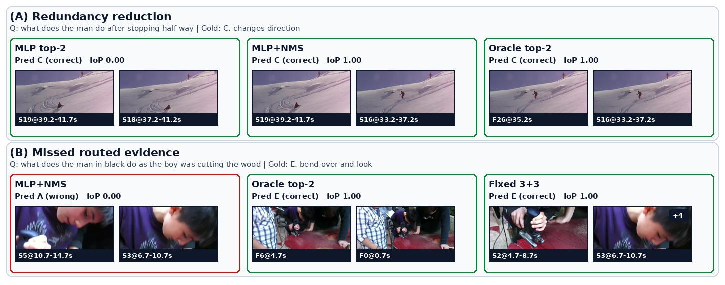
\includegraphics[width=\linewidth]{qualitative_cases.pdf}
  \caption{Qualitative evidence selections on NExT-GQA test. Each row is one question; columns compare evidence selectors. Green borders indicate correct answers and the red border indicates an incorrect answer. Row A shows that temporal NMS reduces redundant evidence: MLP top-2 selects two nearby late segments with IoP 0.00, while MLP+NMS preserves the correct answer and recovers support overlap with IoP 1.00. Row B shows a router failure case: MLP+NMS misses the annotated support and answers incorrectly, but oracle top-2 and fixed 3+3 recover supporting evidence from the same candidate pool and answer correctly. Evidence labels use F/S for frame/segment and include timestamps.}
  \label{fig:qualitative-cases}
\end{figure}

\subsection{Discussion}
The results suggest two practical lessons for grounded VideoQA. First, answer accuracy should not be used as a proxy for grounding: one-segment Qwen evidence already answers many questions correctly, but it often misses the annotated support moment. Second, answerer quality and evidence routing are complementary. Qwen can reason from selected images, but it cannot recover missing temporal evidence; the oracle rows show that much stronger compact grounding is possible from the same pool. Future work should therefore train routers with VLM feedback and represent selected segments with multiple frames or short clips to preserve motion cues.

\section{Limitations}
This study fixes several design choices to keep the evidence-budget comparison controlled. Qwen uses one sampled frame per selected segment, which is efficient but can discard motion cues. Acc@GQA is an evidence-set best-overlap metric rather than the official NExT-GQA single-window evaluator, matching our formulation but requiring separate reporting from official single-span localization. The temporal-supervised router and fixed 3+3 rows are diagnostic references, not the proposed budgeted method.

\section{Conclusion}
Grounded VideoQA should be evaluated as evidence selection plus answer generation. On NExT-GQA, MLP+NMS improves Acc@GQA by 10.0 points over one segment at less than half the fixed 3+3 cost, while oracle top-2 nearly matches the fixed reference. The evidence pool is strong; the remaining bottleneck is routing.

\clearpage
\bibliographystyle{plainnat}
\bibliography{references}

\clearpage
\appendix
\section{Additional Qualitative Examples}
Figure~\ref{fig:appendix-qualitative-cases} provides additional held-out test examples beyond the main qualitative panel. These examples are selected to cover complementary behaviors: fixed-budget context that rescues compact evidence failures, compact oracle support that was available but not selected by the learned router, oracle recovery when learned routing selects the wrong moment, grounded learned successes, and cases where grounding is high but answer prediction is still wrong.

\begin{figure}[p]
  \centering
  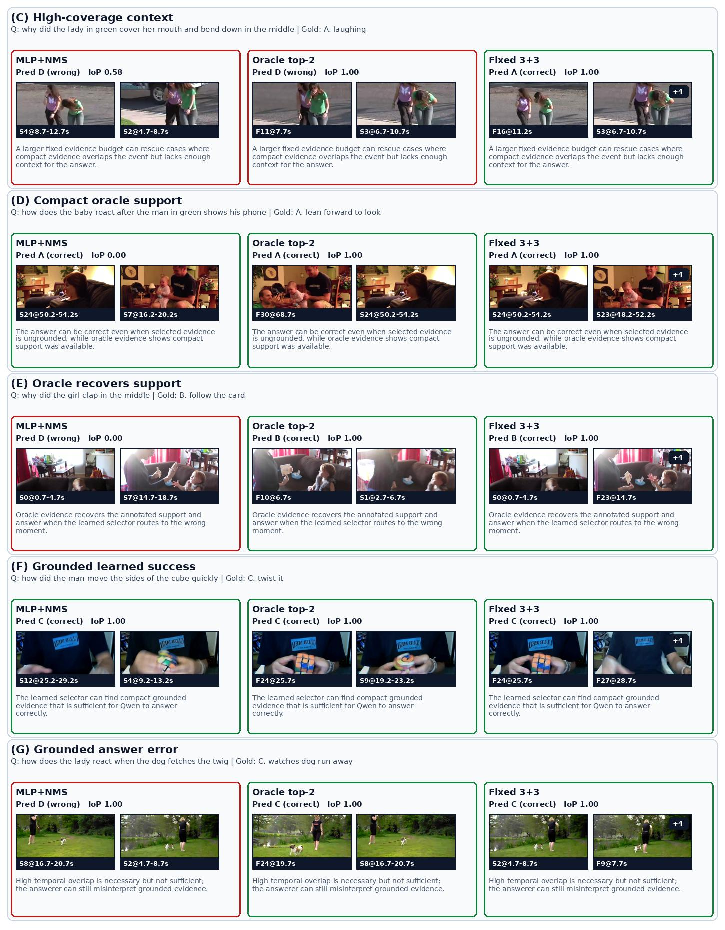
\includegraphics[width=\linewidth,height=0.88\textheight,keepaspectratio]{appendix_qualitative_cases.pdf}
  \caption{Additional qualitative evidence selections on NExT-GQA test. Each row is one question and each column is a selector: MLP+NMS, oracle top-2, and fixed 3+3. Green borders indicate correct answers and red borders indicate incorrect answers. Rows C--G show five complementary behaviors: fixed high-coverage context can rescue some compact-evidence failures; oracle evidence can reveal compact support that the learned selector missed; oracle selection can recover the answer when learned routing selects the wrong moment; the learned selector can also produce compact grounded successes; and high temporal overlap alone does not guarantee a correct answer. Evidence labels use F/S for frame/segment and include timestamps.}
  \label{fig:appendix-qualitative-cases}
\end{figure}

\end{document}
